\documentclass[a4paper,11pt]{article}
\usepackage[british]{babel}
\usepackage[top=1.5cm,bottom=1.5cm,left=1.5cm,right=1.5cm]{geometry}
\usepackage{graphicx}
\usepackage[hyphens]{url}
\usepackage{paralist}
\usepackage{authblk}
\usepackage[noadjust]{cite}
\usepackage[pdftex,colorlinks=true]{hyperref}


% title
\title{Facilitating Collaborative Learning Between Remote Sites Using Large Multi-Touch Devices}

% names
\author[1]{James McNaughton}
\author[2]{Tom Crick}
\author[3]{Andrew Joyce-Gibbons}
\author[4]{Gary Beauchamp}
% \author[5]{}
% affiliation
\affil[1,3]{School of Education, Durham University, UK}
\affil[2]{Department of Computing \& Information Systems, Cardiff
  Metropolitan University, UK}
% \affil[3]{}
\affil[4]{School of Education, Cardiff Metropolitan University, UK}
% \affil[5]{}
% emails
\affil[1]{\protect\url{j.a.mcnaughton@durham.ac.uk}}
\affil[2]{\protect\url{tcrick@cardiffmet.ac.uk}}
\affil[3]{\protect\url{andrew.joyce-gibbons@durham.ac.uk}}
\affil[4]{\protect\url{gbeauchamp@cardiffmet.ac.uk}}
% \affil[5]{\protect\url{}}

\renewcommand\Authands{ and }
\def\UrlBreaks{\do\/\do-}

\date{ }

\begin{document}
\maketitle

% may need to tweak this depending on the chosen journal location!
\begin{abstract}
This paper presents a technical case study and associated research software/hardware underpinning an educational research trial in which large touch-screen interfaces were used to facilitate collaborative interactions between primary school students at separate locations.
As part of the study, an application for supporting a collaborative classroom activity was created for the trial which allowed students at either location to transfer resources to the students at the other via a `flick' gesture.
The experiment required several novel innovations to overcome shortcomings with the application's supporting framework and the technologies used; we also detail how software was used to provide a thorough and robust approach to collation of data relating to the trial, from a research software viewpoint.
\end{abstract}

\section{Introduction}

***{\emph{TC: This feels like it starts too deep, too early -- should be write something more high-level intro here about the use of technology in education, evolving policy? Otherwise, we get right into it straight away...!}}***

Large touch screen interfaces offer many opportunities for collaboration between co-located learners; not only when the interface is shared but when two or more co-located interfaces are networked together to allow for the transfer of materials between them~\cite{kharrufa:2013,kreitmayer:2013}.
As well as presenting valuable pedagogical opportunities, the successful integration of multi-touch tables into usable computer-supported collaborative learning (CSCL) activities presents major challenges both technically and for teacher orchestration~\cite{dillenbourg:2011}. 

This study starts from the viewpoint that collaborative small group learning activities have the potential to lead to substantial learning gains for the participants, more so than activities they completed individually~\cite{odonnell:2013,barron:2008}.
There is a clear role for technology to play in supporting this collaboration, enabling configurations for group work and types of task which are not otherwise possible.
CSCL theory and research emphasises the role of technology in supporting learner participation, knowledge acquisition (information) and knowledge creation (knowledge objects and social practices)~\cite{lipponen:2004}.
Much of the CSCL research base emphasises the importance of face to face interaction and the design of tasks and optimising the participation of learners~\cite{stahl:2014}.

The growing interest in face-to-face collaboration by learners engaged in mutual negotiation of meaning (both procedural and factual) inspired the creation of the SynergyNet project\footnote{\url{https://community.dur.ac.uk/tel.lab/synergynet/}} at Durham University, an EPSRC/ESRC-funded research project to identify important technical and pedagogical challenges in the CSCL domain~\cite{higgins-et-al:2012}.
Important technical challenges included the development of teacher orchestration tools which enabled seamless transition between individual spaces, group spaces and interactive whiteboards; these were respectively termed the private, shared and public spaces in the classroom by Dillenbourg and Evans~\cite{dillenbourg:2011}.
They also identified the potential for a group to share information with other groups, building on the work of Everitt et al.~\cite{everitt:2006}.
However, in this case the mechanism developed did not involve sharing between personal devices such as computers and a multi-touch table; rather, SynergyNet developed tools to allow sharing seamlessly between tables~\cite{hatch:2011b}.

Pedagogically, SynergyNet studies focused on schoolchildren aged 10-11 years old, working in collaborative groups nested within a lab-classroom.
Data was collected on each group and each table as tasks were completed simultaneously.
Data was also collected on the arrangement of the whole class and the teachers’ behaviour whilst supporting the activity.
Studies showed that in tasks completed using multi-touch tables compared to tasks completed using paper-based equivalents, learners showed better uptake of ideas~\cite{mercier:2015}, showed evidence of more sophisticated reasoning  and differences in the amount of time spent in procedural rather than problem-focused talk~\cite{higgins-et-al:2012} in the multi-touch condition compared with the paper-based condition.
Further studies highlighted the importance of the division of roles and showed different patterns of organisational and intellectual leadership in groups using mutli-touch tables~\cite{mercier2014d}, the importance of classroom layout for task completion~\cite{mercier:2014c}, the differences in teacher decision making process when shifting from group to whole-class dialogue~\cite{Joyce-Gibbons:2016}, the development of adaptive expertise among group members~\cite{mercier:2013} and the affordances of the tables to structure representations of reasoning processes~\cite{mercier:2014b}.

The principal limitation of the original SynergyNet study was the fact that research was only ever conducted in the lab-classroom rather than in a real-world school environment, adapting to robust teacher and pupil use and also dealing with the technical challenges of the school's infrastructure.
This is one of the chief priorities of the ongoing research agenda, to bring the tables into authentic classroom settings.

Previous studies have been concerned with how the use of multiple large touch screen interfaces impacts on collaborative education in single environments, i.e. Individual classrooms~\cite{mohammed:2012,kreitmayer:2013,mercier:2015}.
One of the key advantages of collaborative education across multiple locations is that it allows students with a potentially diverse range of knowledge, backgrounds and skills to work together~\cite{kizilcec:2013}.
However, with the opportunities afforded by large networks, both open and closed, for collaboration in education across multiple locations~\cite{daradoumis:2000,mcconnell:2012}, the limitations of co-located interfaces becomes much more apparent.

The use of a touch screen interface offers the opportunity for many novel gestures to intuitively instigate specific actions which can be beneficial for younger users~\cite{kim:2007,wu:2003,rick:2009}.
One such gesture is the `flick' motion~\cite{reetz-et-al:2006}, which is typically used for the movement of materials about an environment with minimal effort.
This gesture can aid collaboration, allowing users to transfer materials to each other without needing to enter each other's interaction space.
 It is possible that the flick gesture could be used, not only for passing content between users on the same interface, but for passing materials to users on remote interfaces.
% The trial built on this possibility and applied it to the transferral of materials between non-co-located locations.

This papers details the work done to support a trial that investigated the impact of using large touch screen interfaces in two separate locations, specifically with UK Key Stage 2 classrooms, on collaborative interactions and its impact on education. 
Furthermore, this paper represents a valuable case study of the technical aspects of implementing a research trial using these multi-touch devices, examining how technology was used to collect the wide range of research data, as well as the technical challenges faced.


\section{SynergyNet}

As part of the wider SynergyNet project, a software framework\footnote{Available on GitHub: \url{https://github.com/synergynet}} was developed to support applications designed for multi-touch interfaces.
This SynergyNet framework allowed any item in its supported applications to be moved and manipulated by users through common multi-touch gestures, as well as supporting communication between multiple interfaces via a network connection.
The framework supports several different methods of transferring materials between instances of its apps; the use of networked interfaces allowed media-based content to be easily shared between multiple users, allowing both intra- and inter-group collaboration as show in early SynergyNet studies~\cite{mercier:2014b}.
This feature was presented as a capability of the teacher orchestration tools within the SynergyNet classroom which allowed the teacher to decide when to instigate the transferral of content~\cite{alagha-et-al:2010,mercier:2016}.
An additional capability, called `Network Flick' was developed which allowed learners working at each table to ‘flick’ content (transfer content from one table to another by using a flicking gesture)~\cite{reetz-et-al:2006}.
Whilst technically this was achievable in the lab-classroom, the co-location of all groups resulted in a study design which made the gesture’s capabilities pedagogically ineffective.

Recent research building on the outcomes of the SynergyNet project has focused on developing the use of multi-touch tables for group work in multiple schools, resulting in the network flick gesture of the framework now having a pedagogical grounding and purpose.
The project this research forms part of has resulting in the collaboration with two schools which are geographically distant in the UK (approximately 300 miles apart) -- one near the city of Durham in the north-east of England and the other near Caerphilly in south Wales.
Despite their distance, the areas share an interesting common industrial heritage; specifically, they were at the heart of the coal mining industry which powered the industrial revolution.
Latterly both areas have experienced significant post-industrial economic trauma with the closure of the mines and de-industrialisation.
The impact on the children living in these former mining communities has led to a dislocation with their environment as they grow up with little or no first-hand knowledge of mining, although are aware of the cultural heritage of the community (as well as their families) -- both participating schools reported that learners in their schools were aware of mining as a ‘heritage’ activity but did not relate it to their lives now or consider it relevant to people of their age.

The project sought to address this by establishing shared group work through the network flick gesture; the multi-touch tables were used to support children in collaborative group tasks previously intended to be completed by a single group assumed to be working in a single location.
However, to try and increase the sense of common history and shared endeavour, the task was split with children in both locations being asked to work together to solve the problem, communicating via video conferencing software (visual and verbal) as well as by sharing data and resources via the network flick gesture.
This paper primarily focuses on the technical challenges in the design and implementation of the framework from a research software engineering perspective, identifying key issues and constraints; future work, already in progress, will focus on the wider pedagogical and social implications of the study.


\section{Technical Challenges}

***{\emph{TC: Can we identify any more Technical Challenges? They're all largely network-related; anything to do with the user interface, HCI, weird artefacts with using the devices, etc?}}***

\subsection{Network Flick}

***{\emph{TC: Must be a corpus of work we can reference here, esp. in regards to games and flick gestures? Let me look...}}***

The network flick gesture is built upon the metaphor of pushing items around on a low-friction surface (such as ice), now a common feature of many mobile and touch screen devices.
A small amount of initial effort can allow the item on which the force is being exerted to travel a great distance, whereas friction can be applied to decelerate flicked objects over time which is useful for both helping users keep control of items (i.e. so they do not continue to travel indefinitely at high speeds after being flicked making them difficult to grab and stop) and for making the behaviour of the item better match its real world equivalent from the metaphor of sliding objects on ice.

The networking element of this gesture appears when users flick a content item in the direction of the interface to which they wish to send content; the item travels off the side of the initial interface and appears on the target interface as shown in Figure~\ref{fig:FlickExample}.
Flicking in a direction where there is no connected interface results in the item bouncing off the interface boundary, as would be expected in the real world.

\begin{figure}[h]
 \centering
   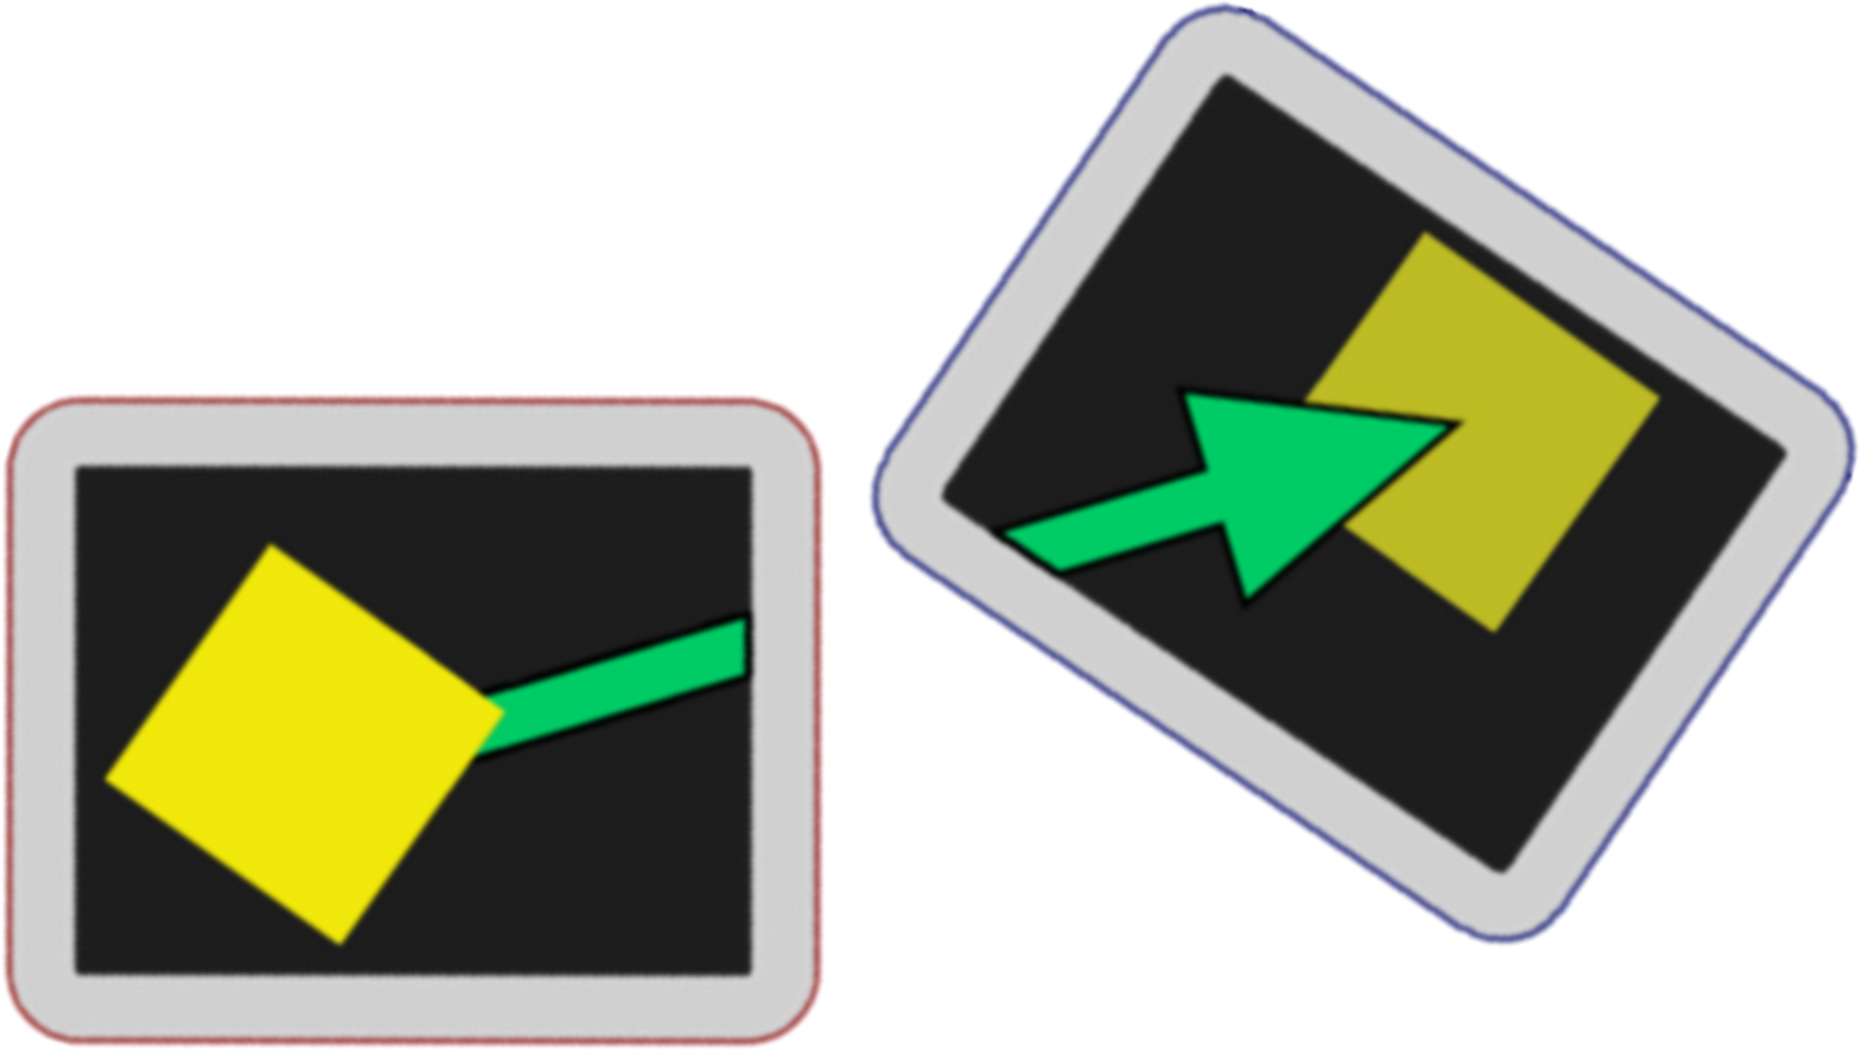
\includegraphics[width=0.75\textwidth]{figures/flickexample.png}
   \caption{The use of the network flick gesture to transfer content between co-located interfaces.}
   \label{fig:FlickExample}
\end{figure}

When the item arrives on the target interface, the framework can use its knowledge of the interface locations to ensure the item appears in view from the appropriate direction of the source interface.
This is intended to aid users in easily identifying from where newly arrived content items have been sent when the interfaces are co-located.
The use of a flicking gesture not only informs users on recipient interfaces of the origin of transferred items but also creates an intuitive way of sending and sharing content.
Users are capable of choosing their recipient through the direction of the flick and thus initiate the transfer simply by moving the item in that direction and releasing it.
This is intended to reduce the cognitive load usually required to move content between interfaces.
The potential benefit of this approach, by having a simple method to move content between interfaces, users will be more willing to share items as there is less of a barrier to sending and receiving.

Though the network flick gesture has a number of potentially benefits, little use has previously been found for it; the feature has been present in the SynergyNet framework since its earliest versions, but very few apps utilise it.
While some apps that require the transfer of materials between interfaces do support the gesture, most encourage users to use other, more traditional, methods of sharing contents (such as placing items in shared areas or through using a context menu).

***{\emph{TC to find some more citations for below...}}***

Previous studies have investigated the human-computer interaction and affective computing aspects of the network flick gesture, but none of these have entailed its use in a classroom environment.
Typically, classroom-based studies with SynergyNet have utilised a remote teacher interface to orchestrate the transferral of content~\cite{joycegibbons:2016}.
Though the gesture is often used in the warm-up and cool-down sessions (to get participants used to interacting through the touch screen devices and as a form of play reward) during previous studies with UK Key Stage 1 and 2 students and has always been well received, there has been little data collected on its use by pupils as part of classroom activities.
% Where it has been used, the network flick has always been performed to transfer content between two co-located interfaces previously.

\subsection{Co-Location}

The majority of SynergyNet features have been developed with co-located interfaces as the intended environment for their use.
Often in the past, the apps developed for SynergyNet and key features for the framework itself have been created for specific research studies.
As all of these studies have taken place in single environments, the features and apps of the framework were built assuming co-located environments.
Though efforts were made to ensure that the SynergyNet framework was dynamic and adaptable as possible, functioning across multiple environments in separate locations was not a priority during its past development and as a consequence there are several shortcoming in the system design.
This is apparent in both the visual and functional design of the framework and apps.

Many of the interfaces presume that users will be together in the same environment and able to see each other's screen directly; this has a large impact on the design of visual elements, such as the menus; for example, the menu used by teachers to transfer content in previous studies assumes that the teacher is able to see pupil's interfaces so that they can choose which group's work they can display to the class.

The network flick gesture itself makes an assumption about its use which results from its intention for previous use between co-located interfaces: that users will know where their target interface is in relation to them.
However, this knowledge can also be made available to users even when their target interface is in a remote location.
The implications of not directly seeing the target interface when performing a network flick gesture are one of the key focuses of this new strand of work.

%\subsection{Virtual Private Networking}
\subsection{Networking}

As many of SynergyNet’s networking features -- including the network flick gesture -- are dependent on the devices being on the same local network, it became apparent that the most time-effective approach would be to emulate a local area network across a wider network (i.e. the internet).

This course of action was decided upon as supporting direct communication across the internet would have required several of the framework’s features to be totally redeveloped which was not feasible in the time-frame of the study (as well as issues of approaching the end of the academic year where classes would have the availability to participate).
After investigation, the most effective way to emulate a LAN was to utilise a virtual private network (VPN), allowing many of the features of a local network that SynergyNet relies on (such as shared folders), whilst still communicating across the wider internet.

% removed citation~\cite{zerotier:2016}
Though many VPN solutions are available, Zero-Tier\footnote{\url{https://www.zerotier.com}} was selected to provide network virtualisation services.
This low-cost VPN solution is not a typical VPN, but fulfilled all the criteria needed to support the majority of SynergyNet’s networking features over the internet.
As only a small number of machines required to be connected to the same network in the trial (i.e. two; one touch-screen table-top interface for each site; the tablets used in the trial for the video conferencing did not need to be on the same network as the table-top interfaces and could just function as-is over the internet) it was not necessary to use feature-rich VPNs; though Zero-Tier may not be as secure as other VPN options, the trial did not involve any private data being transmitted between the two sites.

It was originally intended that all devices used in the trial could be connected to the internet via the schools' own network infrastructure (both the tablets and table-top interfaces are capable of using wireless connections).
However, during preparation for the trial it was discovered that the firewalls at both of the schools were explicitly blocking outbound VPN traffic relating to Zero-Tier.
The use of the Zero-Tier VPN had been tested in environments with strict firewall policies (e.g. University networks) and had operated as expected; however, it appears that the school firewalls were locked down much more than anticipated, with extremely limited outbound connections allowed through the firewall.
This meant that SynergyNet could not operate when connected to the Zero-Tier VPN when connected through the schools’ networks.
Whilst adding exceptions to the firewalls would have allowed the VPN connections to function correctly, this was not feasible due to administrative issues with approval via the school and local education authority; therefore an alternative method of connecting to the internet was required.

\subsection{Mobile Connectivity}

Due to permission issues with the schools' own network infrastructure, an alternative method of connecting to the internet that would allow the table-top interfaces to function was identified using pay-as-you go 4G mobile ``dongles''.
These could be connected via USB to the two table-tops to allow them to connect to the internet through a relatively fast mobile connection.
However, do to the remote locations of each school, it was difficult to find decent coverage using a single mobile network, so the interfaces at both sites were connected to the internet through two different 4G providers.
This had no noticeable impact or latency on the connection and allowed the instances of SynergyNet on both table-tops to interact quickly and with minimal data loss (for example, failed transmissions of messages between the instances would result in flicked items never arriving on their target device).
% As the table-top interfaces were only to be used for the trial and the app's network usage is minimal, pay-as-you-go plans sufficed.
The app only sends data when first finding other instances of the app and when a content transfer occurs; the first time any content is sent it is moved to the shared area on the network; afterwards, all subsequent transfers point back to the same item in the shared area, treating it like a cache.
In addition to the trial's app, remote desktop controlling software, VNC, was also briefly used to and ensure both tables were set up on each site correctly before the trial started.

A 4G connection may not be as secure as using the school network but data to and from the VPN was end-to-end encrypted ensuring it would be secure; furthermore, no sensitive or personal data was being transmitted between the tables.
% The video conferencing tablets used the school networks which would have provided an adequately secure connection.

\subsection{Multi-casting}

SynergyNet up until now had used multicast service discovery as a method of finding other running instances of the framework on a network.
However, many VPNs do not support the User Datagram Protocol (UDP) that SynergyNet employs.
Thus to accommodate this VPN constraint, the framework was modified to work purely through the more widely supported Transmission Control Protocol (TCP).
This change meant that SynergyNet could no longer automatically detect other instances; at least one instance would need to be informed of the IP address of the other instance.
To support this a user interface was developed which allowed for the user to allocate participating device's IPs on the network.
This update was initially a change at the app level but has since been integrated into the framework so that all apps on the latest version of SynergyNet~\cite{hatch:2011} can work across VPNs easier.

\subsection{Other Technical Considerations}

Both the design and the technical underpinnings of the SynergyNet framework and its apps been limited by the assumption of use across only co-located interfaces.
The use of single environments in the past meant that the framework was always deployed across a single Local Area Network (LAN) in all studies; as there was no need previously for the framework to be able to work across anything beyond a LAN many of the features are not capable of functioning across the wider internet.

% remove refs: ~\cite{igniterealtime:2016} and ~\cite{hazelcast:2016} 
Despite the intention of being used solely across LANs in the past a large amount of the framework's networking capability was built in such a way that it could easily function across the internet.
The use of third party libraries such as OpenFire\footnote{\url{https://www.igniterealtime.org/projects/openfire/}} (a real time collaboration (RTC) server that uses the widely adopted open protocol for instant messaging, XMPP/Jabber) and Hazelcast\footnote{\url{https://hazelcast.org/}} (an open source in-memory data grid based on Java for simplified distributed computing) mean that the framework can use several different protocols across wider networks for communicating messages to each other.

However, there are some network features that are solely limited to LAN; an example of this is how media content is transferred between instances of the framework.
The framework uses a shared network location as a form of cache, which was beneficial in the past as it was simple to implement and gave teachers a single location to collect the files used in a lesson for use in future lessons.
The secure use of a shared network location across a wider network, such as the internet, is inadvisable without precautions due to data security and latency of such a technique.
It was therefore a requirement that some development work took place prior to the trial taking place to allow the framework, or at least the app used, to function over the internet as the two locations used would not be able to share a typical LAN.

\section{Example SynergyNet Experiment: Two UK Primary Schools}

***{\emph{TC: Are we aiming to provide a methodology here, or an overview to the approach to aid understanding of the technical aspects for this paper?}}***

For this trial, two groups of UK Key Stage 2 students (aged 9-10 years old) at separate locations were encouraged to work together on a classroom activity.
As previously mentioned, one group was situated in a school in the north-east of England and the other in a school in South Wales.
It was decided that the trial should take place near to the end of the academic year (summer term) to cause as little disruption to the teaching schedule as possible.
The design of the trial was built on previous SynergyNet studies which meant that a lot of the preparation was already in place (i.e. the hardware, the supporting software framework and the tasks to be carried out).
However, previous SynergyNet studies all took place in a single classroom environment, the trial's use of multiple locations meant that there were several new challenges in the set up to overcome during this short lead in time.
Each group was allocated a large touch-screen table-top device (Samsung SUR40s) to work together on the collaborative activity; the landscape nature of the interfaces was chosen to allow multiple students to work around the devices at the same time.
The two devices were networked together to share content between them, specifically through the network flick gesture.
To allow the teams to communicate and to give them a direction to focus their flick gestures towards, a tablet was positioned by the tables along one side at both locations, using video-conferencing software (Skype) to allow the teams to see each other and communicate verbally.
The tables were configured so that flicking items towards the tablet screen would transfer them to the remote table; this meant each table considered the other to be co-located.
This was achieved by configuring the tables so that they were virtually positioned next to each other (with the sides on which the tablets were placed being parallel to each other), when in reality they were on opposite sides of the country.
With students passing items towards their `window' to the other team, the metaphor of physically pushing items towards another interfaces was maintained.

Virtually positioning the tables side-by-side also meant that the entire edge of the tables with the tablet on (one of the longer edges of the widescreen aspect ratio interfaces) could be used as the target for network flicks.
If the two tables were configured to use their real-life locations in relation to each other, the size of the boundary where a network flick could be trigged (i.e. that points to the remote table) would be less than a pixel at the distance between the two locations.

Another benefit to this configuration of the tables being placed virtual side-by-side relates to the behaviour of the transfer.
Normally a realistic effect is employed where the time taken for items to transfer is calculated by the time it would take them to travel the gap between the interfaces at the speed of the item before it left its source interface (ignoring deceleration).
This is a useful behaviour for co-located interfaces as it bolsters the metaphor of real objects being pushed around the environment.
However, this behaviour would not be suitable with the interfaces using their real world locations in the trial as it would take a long time (likely longer than the trial sessions, even with the fastest flick the interfaces are capable of identifying).
With the virtual distance between the tables set to be as small as possible the flick behaviour had the effect of items travelling the distance from one interface to the other via the `window'.
% The positioning of the tables was set through configuration.
% Other changes to make the framework ready for the trial required some new developments.

%\subsection{Flick Mysteries}

***{\emph{TC: Do we need to explain this a bit more? (maybe not...)}}***

The selected collaboration task for this trial was {\emph{Mysteries}}; a classroom activity where students use a selection of clues, such as snippets of text and images, to solve a problem or come to a conclusion about an open question; this task has been used in several previous SynergyNet studies~\cite{mercier:2013,mercier:2014,mercier:2015}.

\begin{figure}[h]
 \centering
   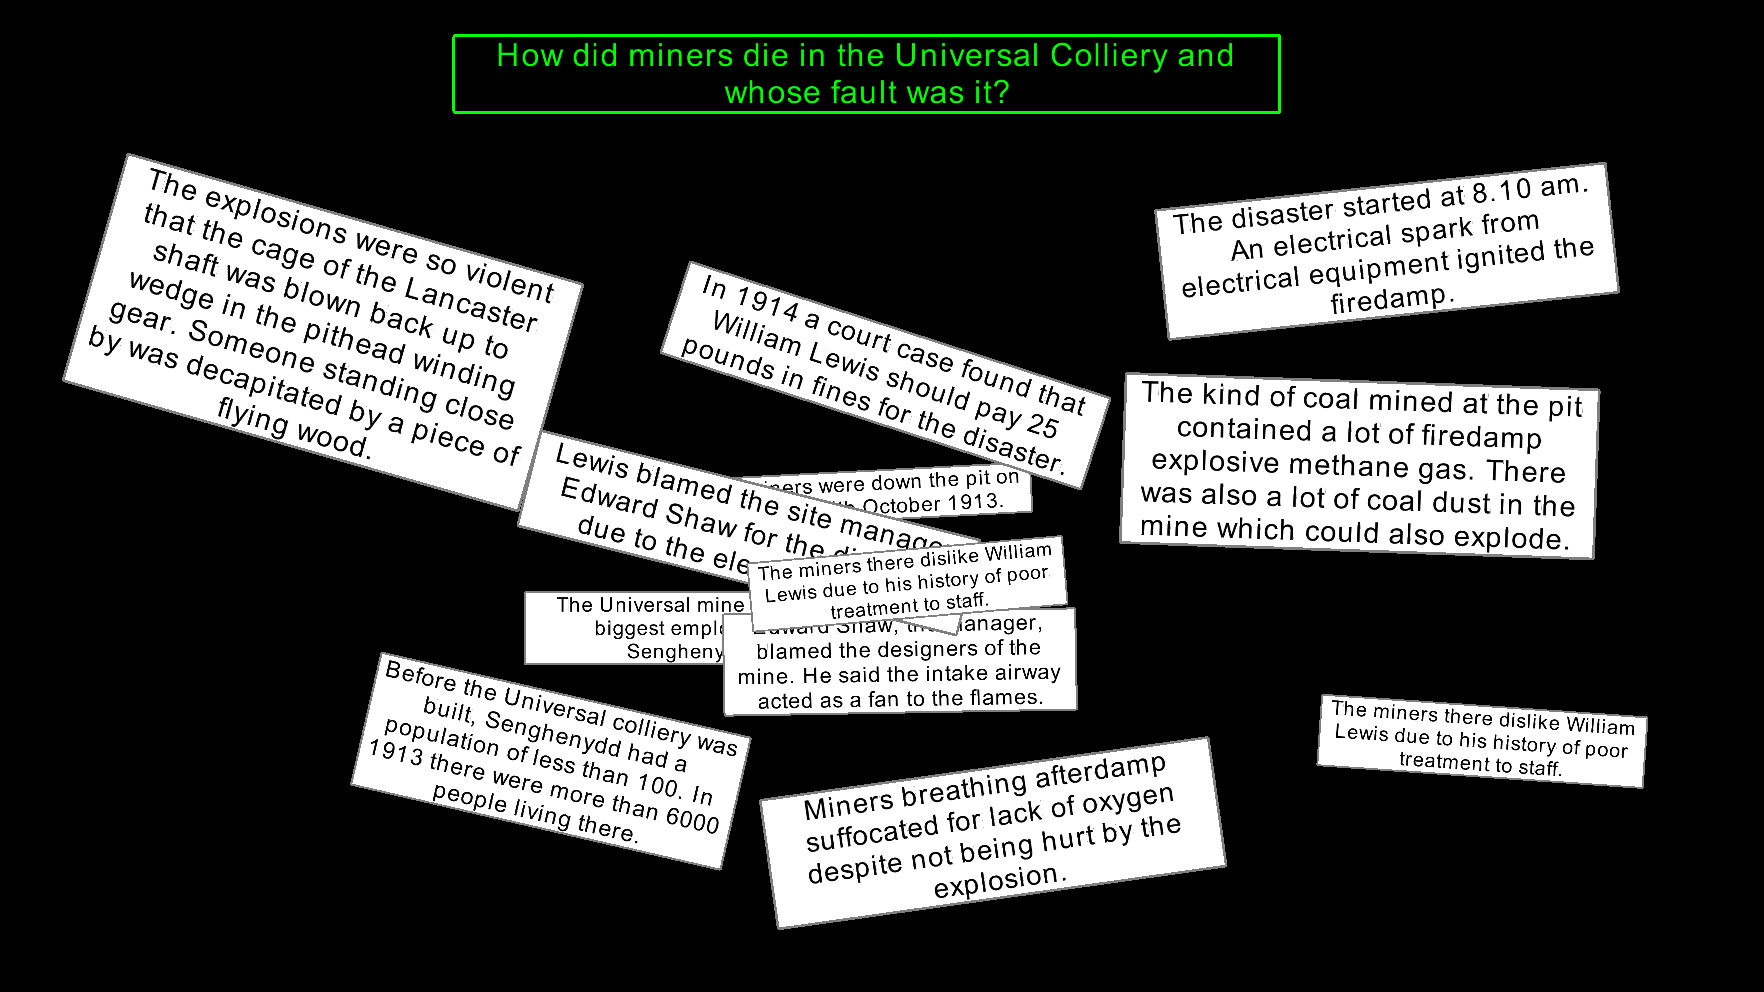
\includegraphics[width=0.75\textwidth]{figures/flickmysteryexample.png}
   \caption{The SynergyNet mysteries app with task content used in the trial.}
   \label{fig:FlickMysteryExample}
\end{figure}

Though {\emph{Mysteries}} is an existing task supported by several apps for the SynergyNet framework, none of them utilise the network flick gesture.
This required the creation of a new app which would manage the loading of the materials in a dynamic way (i.e. text snippets from a simple XML file and media from any other files in a folder, although video and audio clips are supported by the app only images were used in the trial alongside the text snippets to reduce potential confounding factors) and allow them to be transferred through the network gesture.
The dynamic content system allowed for the app to be easily configured so that each site would have a different selection of clues for each mysteries task, forcing them to share content with the students at the remote location.
Figure~\ref{fig:FlickMysteryExample} shows the app built for the trial with content relevant to the task dynamically-generated from an XML file ready for transfer via the network flick mechanism.


\section{SynergyNet Data} 

To collect relevant experimental data, the trial consisted of four sessions, each taking an average of 20 minutes.
Throughout these sessions a wealth of data was collected in the form of recordings; these recordings were annotated and coded in a robust and consistent manner by the project team to provide quantitative data of the interactions.
This quantitative data could then be used alongside quantitative information, like observations made on the recordings, to generate the findings for the trial.
 
%\subsection{Data Collection}

Screen recording software was used to collect data during the experiment; this software was installed on both tablets allowing both sides of the video conferencing software used for communication between the groups to be recorded.
In addition to this,stand-alone cameras were used at both locations to record in high-detail interactions with and around the table-top interfaces.
Unfortunately, because SynergyNet uses OpenGL (a cross-language, cross-platform API for rendering 2D and 3D vector graphics) for its visual output, it was not possible to capture video easily from the screen for two main reasons: it is problematic if we wished to use a secondary device that the output is mirrored to, as the set-up on the table-top interfaces that used the display is integrated into the device and changing the visual output configuration is limited; also, it would impact on the performance of the device, which is not an acceptable occurrence as performance should be priority to ensure fewer barriers to intuitive interaction.

%\subsection{Data Collation}

%With the trial now completed the next step was to collect meaningful data from the videos recorded.
While qualitative information can be collected from this videos (and trial orchestrator's observations made during the trial) the intention was to capture quantitative data to evaluate the use of network flick gestures between non-co-located interfaces for classroom activities.

\begin{figure}[h]
 \centering
   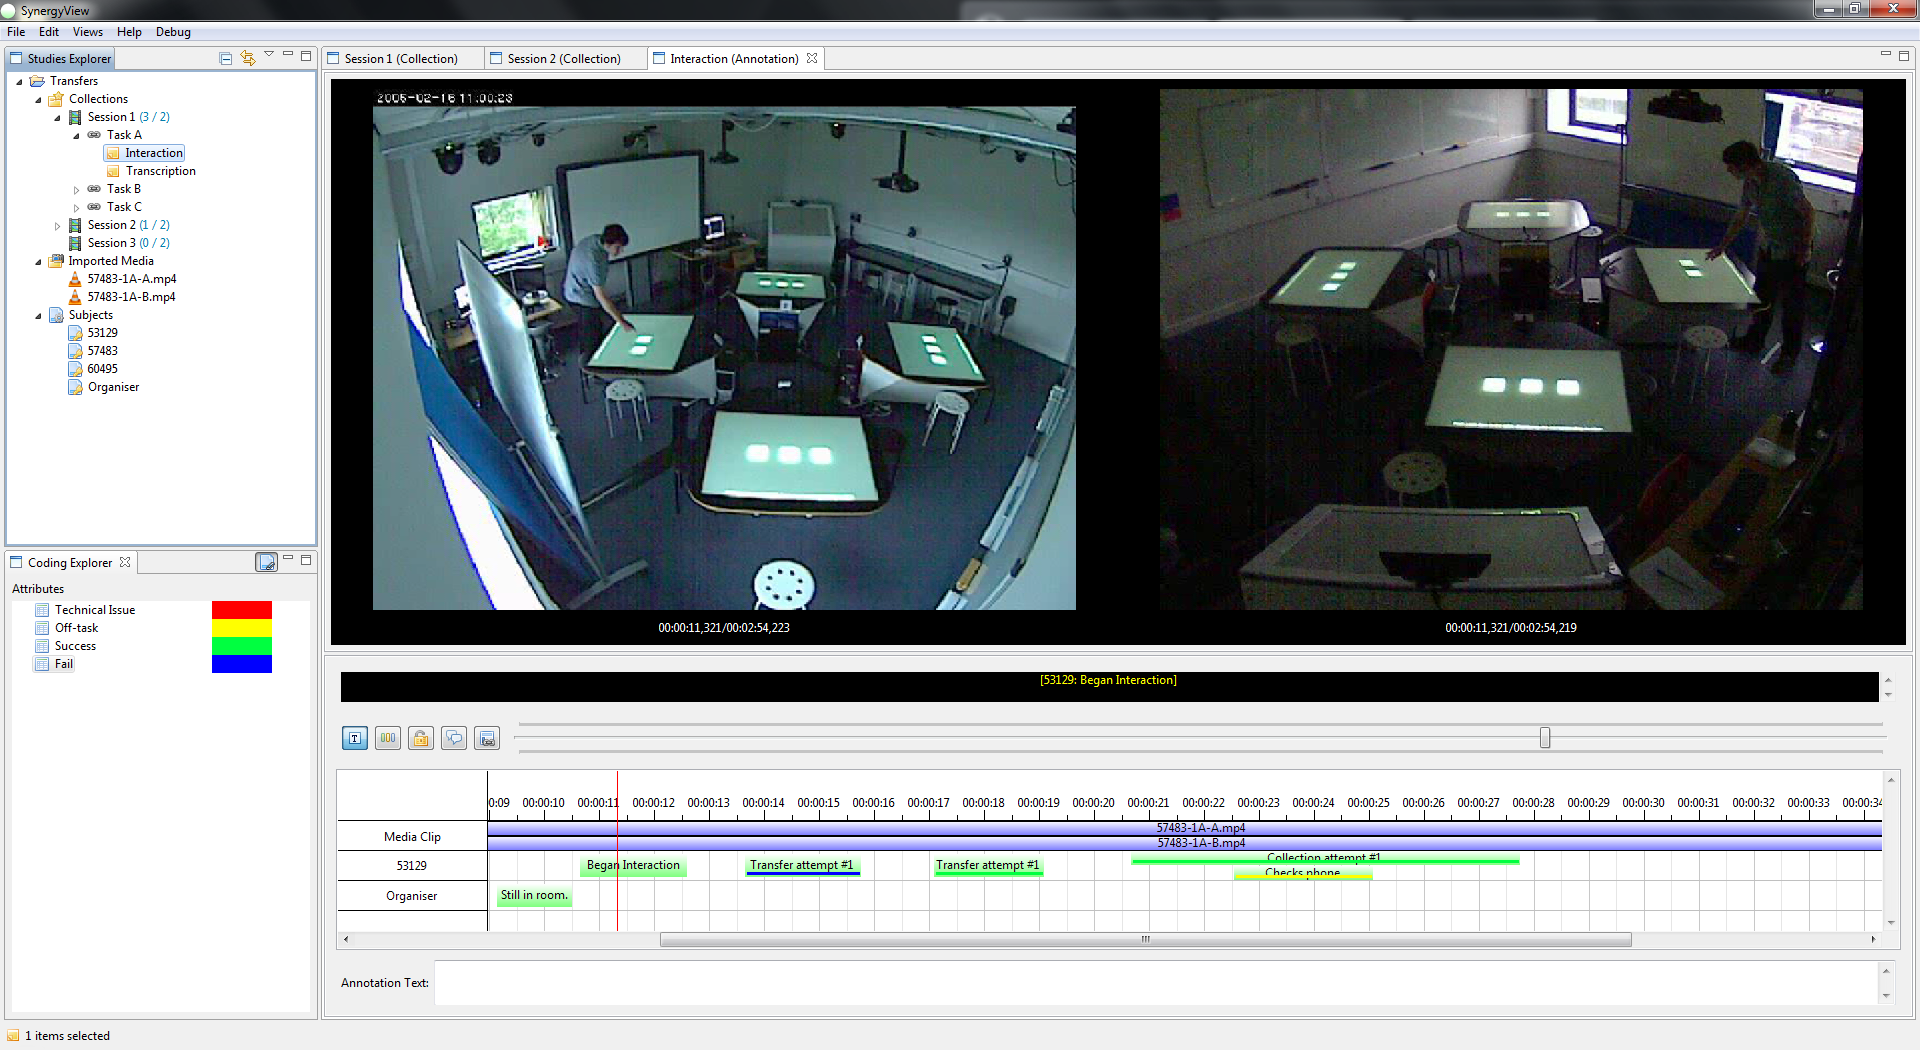
\includegraphics[width=0.75\textwidth]{figures/synergyviewexample.png}
   \caption{The SynergyView video time-line analysis tool in use.}
   \label{fig:SynergyviewExample}
\end{figure}

SynergyView~\cite{kyaw:2010} is a time-line analysis tool where multiple videos can be annotated together over time with each annotation being tagged with a wealth of information (such as the subjects in the video they relate to or a type of recurring event seen in the trial).
Information on these annotations, such as their frequency, total times and average times can then be exported in a cross-tab format for analysis.
The intention was to use SynergyView to annotate the videos from both groups in the trial session together (once synced).
As multiple sessions took place during the study where different groups of students participated there were several sets of videos to annotate together.
The resulting cross-tabs of information relating each of the sessions could then be collated and analysed as one large dataset.
The tool allows for the exporting and importing of annotations made during the data collation, thus several researchers worked together to annotate the videos; the ability to share annotations allowed for this to be collaborative effort made between sites. 
This quantitative data, in addition to other more qualitative observations made during the sessions and from the videos, provide crucial insight into the use of the trial's configuration of technologies in the classroom.


\section{Conclusions and Future Work}

***{\emph{TC: Lots of short sentences here; are all of these lessons learnt applicable to the technical outcomes of this paper? They are generally good/useful, but we need to hit the technical issues much harder here. I will need to work through this section again after Gary has had a go.}}***

% removed citation~\cite{hatch:2011}
Analysis of the outcomes from the study, particularly the wider pedagogical and social implications, are now underway and will be reported on in future papers; however, the process of preparing, running and collecting data from the trail has produced several tangible deliverables.
Though SynergyView has been used before in previous research this is the first time it has been documented as being used across multiple sites.
Another deliverable is the Flick Mysteries application for SynergyNet; this application is now available through the SynergyNet repository\footnote{Available on GitHub: \url{https://github.com/synergynet}} for any researcher who wishes to replicate the trial.
The app is designed to make configuration straightforward, as well as allowing for the creation of new trials based around different classroom tasks.

The adaptation of the SynergyNet framework's networking features to work through a VPN is another tangible outcome of this work.
This now allows the framework, and any of the applications it supports, to be used across multiple sites, facilitating further research trials in collaboration between remote sites using natural user interfaces.
Though the trial used a set of specific multi-touch table devices, the portability of the SynergyNet framework allows for it to be run on a range of different devices, including Windows tablets which are widely available.
This affords the opportunity to deploy similar trials into a wide range of environments in the future with little reliance on the bespoke and expensive hardware available.
Furthermore, the challenges of getting equipment to, then setting it up at, multiple locations can be overcome in future studies.

Also arising from the technical work were several approaches to setting up the required equipment in schools, particularly around networking and connectivity.
The use of 3G and 4G network connections to avoid the difficulties of locked-down school networks may prove to be useful in future studies but great caution should be exercised.
In the study described above, no personal or sensitive data was sent through the network connection and all information was encrypted via the virtual private network.
However, the use of a school's network which has been verified as secure is always preferable where feasible, providing improved connectivity and resilience.

From a data collection perspective, the SynergyView tool was updated prior to the collation to remove several minor bugs and ensure it would work on a range of modern operating systems.
Previously the tool had failed to work due to its dependence on third party software no longer supported in the most recent versions of Windows and Mac OS.
The updated version of SynergyView is now available for any researcher who wishes to utilise it through the GitHub repository.

% The researchers at the two separate institutions who carried out the trial (Durham University and Cardiff Metropolitan University) were able to share their work regularly which ensured duplication of effort was minimised throughout the video annotation process.
% This led to the quicker production of usable video annotations than would have otherwise be possible.

%\subsection{Future Work}

***{\emph{TC: We need to tail this more strongly to identify the key technical contributions, as well as linking to any emerging policy?}}***

With the changes to the framework made as part of the trial, SynergyNet is now better suited for use across the internet where a VPN is set up appropriately.
This allows for the tables used in the trial to be re-deployed anywhere where there is an acceptable 3G/4G signal or with an alternate network connection where the network is configured appropriately.
This will enable for further trials using the framework and the tables used in the trial at separate sites.
These further trials may involve following up any discoveries uncovered as part of the trial's data-analysis.

***{\emph{TC: Check refs, maybe a few more options here from both GB's and TC's previous work?}}***

\bibliographystyle{ieeetr}
\bibliography{jors2016}

\end{document}
